\chapter{Meiji Modernity: Science, Superstition and Folklore Studies}

\section{The problem of the modern}

After 1868 the Meiji state set out to make Japan a modern nation on the Western model
(``civilization and enlightenment'', \ja{文明開化}). Belief in yōkai, fox possession and
curses was now labelled \textbf{superstition} (\ja{迷信}, meishin), an obstacle to
progress and an embarrassment before Western eyes. Yet this is also the period in which
yōkai were \emph{studied}, \emph{collected} and redefined as national heritage. Two figures
represent the two attitudes.

\begin{center}
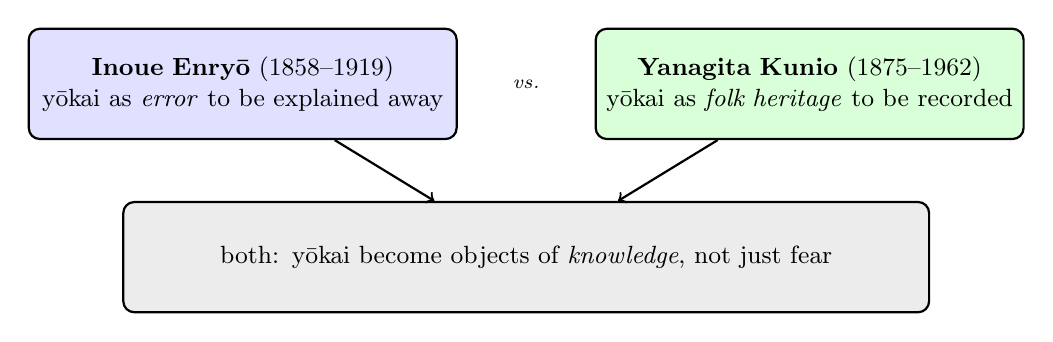
\begin{tikzpicture}[b/.style={draw, thick, rounded corners, align=center, font=\small, text width=5.2cm, minimum height=1.4cm}]
  \node[b, fill=blue!12] (i) at (-3.6,0) {\textbf{Inoue Enryō} (1858--1919)\\yōkai as \emph{error} to be explained away};
  \node[b, fill=green!15] (y) at (3.6,0) {\textbf{Yanagita Kunio} (1875--1962)\\yōkai as \emph{folk heritage} to be recorded};
  \node[b, fill=gray!15, text width=10cm] (m) at (0,-2.2) {both: yōkai become objects of \emph{knowledge}, not just fear};
  \draw[->, thick] (i) -- (m); \draw[->, thick] (y) -- (m);
  \node[font=\scriptsize\itshape] at (0,0) {vs.};
\end{tikzpicture}
\end{center}

\section{State policies against ``superstition''}

\begin{itemize}
  \item \textbf{1868}: separation of kami and Buddhas (\ja{神仏分離}); in some areas a
        violent movement to ``abolish Buddhism and destroy Shakyamuni'' (\ja{廃仏毀釈})
        destroyed temples and images.
  \item \textbf{1872--74}: bans on mountain ascetics (shugendō), certain spirit mediums and
        healers; exorcisms and fox-possession cures discouraged.
  \item State Shinto: shrines reorganized as national institutions for emperor worship,
        distinguished from ``religion'' and from ``superstition''.
  \item Schools taught science and hygiene; newspapers mocked rural beliefs.
\end{itemize}

\begin{remark}
Ironically, the same state promoted a mythology of its own: the divine descent of the
emperor from Amaterasu (Week 3). What counted as ``superstition'' and what counted as
``national tradition'' was a political decision.
\end{remark}

\section{Inoue Enryō: ``Doctor Yōkai''}

Inoue Enryō was a Buddhist philosopher trained at Tokyo Imperial University, founder of
the school that became Tōyō University, and the inventor of \textbf{yōkaigaku}
(\ja{妖怪学}, ``yōkai studies''). He collected thousands of reports of strange phenomena
from across Japan and published the massive \emph{Lectures on Yōkai Studies}
(\emph{Yōkaigaku kōgi}, 1893--94). His nickname was \emph{Yōkai hakase} (``Doctor Yōkai'').

\subsection{His classification}

\begin{center}
\begin{tikzpicture}[
    level 1/.style={sibling distance=7cm, level distance=1.6cm},
    level 2/.style={sibling distance=3.4cm, level distance=1.8cm},
    every node/.style={draw, thick, rounded corners, align=center, font=\small, fill=white, text width=2.8cm},
    edge from parent/.style={draw, thick, ->}]
  \node[fill=purple!15] {yōkai (strange phenomena)}
    child { node[fill=gray!15] {\textbf{false yōkai}\\\ja{虚怪}}
      child { node {\emph{gikai} \ja{偽怪}\\artificial: hoaxes, tricks} }
      child { node {\emph{gokai} \ja{誤怪}\\mistaken: misperception, coincidence} } }
    child { node[fill=yellow!25] {\textbf{real yōkai}\\\ja{実怪}}
      child { node {\emph{kakai} \ja{仮怪}\\provisional: natural phenomena not yet explained} }
      child { node {\emph{shinkai} \ja{真怪}\\true mystery: the ultimate unknowable} } };
\end{tikzpicture}
\end{center}

\begin{itemize}
  \item Most reported yōkai, he argued, were hoaxes or mistakes: a ``ghost'' is a willow
        swaying in the dark; a fox-fire is phosphorescence; fox possession is a nervous
        disorder.
  \item \emph{Kakai} could be explained by science in time (electricity, magnetism,
        psychology).
  \item Only \emph{shinkai}, the true mystery, remained, and for Inoue this was the
        profound reality that Buddhist philosophy points toward. His aim was not to destroy
        wonder but to purify it: clear away superstition so that real religious awe could
        be felt.
\end{itemize}

\begin{example}[Kokkuri-san]
In the 1880s a table-turning craze swept Japan: \emph{kokkuri-san} (\ja{狐狗狸さん},
written with the characters for fox, dog and tanuki), a version of the Western table-tipping
séance brought by sailors. Participants put their fingers on a coin over a sheet of
characters and asked questions. Inoue investigated and explained it as unconscious muscle
movement (the ideomotor effect). Kokkuri-san is still played by schoolchildren and
reappears in J-horror.
\end{example}

\section{Lafcadio Hearn}

\textbf{Lafcadio Hearn} (1850--1904; Japanese name \textbf{Koizumi Yakumo}, \ja{小泉八雲})
was a Greek-Irish journalist who arrived in Japan in 1890, taught English in Matsue,
married a Japanese woman (Koizumi Setsu, who told him many of the stories), and became a
Japanese citizen.

\begin{itemize}
  \item \emph{Kwaidan: Stories and Studies of Strange Things} (1904) retold ghost
        stories in English: ``Yuki-onna'' (the snow woman who marries a woodcutter),
        ``Mujina'' (the faceless \emph{noppera-bō}), ``Mimi-nashi Hōichi'' (the blind
        biwa player whose body is covered in sutras except for his ears, which ghosts tear
        off), ``Rokuro-kubi''.
  \item Hearn romanticized ``Old Japan'' as a disappearing world of gentle beliefs, in
        contrast to Meiji modernization. He is still celebrated in Matsue.
  \item Kobayashi Masaki's film \emph{Kwaidan} (1964) adapted four stories with stylized
        sets.
\end{itemize}

\begin{important}[Hearn and Orientalism]
Hearn wrote for Western readers who wanted an exotic, spiritual Japan, and his books
became sources for Japanese readers too (some stories are now known in Japan mainly via
Hearn). He is a useful case of how an outsider's romantic gaze can shape a tradition's
self-image (connect to Said, discussed in EASIA 201R).
\end{important}

\section{Yanagita Kunio and folklore studies}

\textbf{Yanagita Kunio} (\ja{柳田國男}) was an elite bureaucrat (in the Ministry of
Agriculture and Commerce) who became the founder of Japanese \textbf{folklore studies}
(\ja{民俗学}, minzokugaku).

\subsection{\emph{Tōno monogatari} (1910)}

\begin{definition}[Tōno monogatari]
\emph{The Legends of Tōno} (\ja{遠野物語}) is a collection of 119 short accounts of local
beliefs and experiences, told to Yanagita by Sasaki Kizen, a young man from the town of
Tōno in Iwate prefecture, and written down in elegant literary Japanese. It includes
\emph{kappa}, \emph{zashiki-warashi} (house-spirit children who bring prosperity),
mountain men and women, kamikakushi, fox tricks and ghosts.
\end{definition}

\begin{itemize}
  \item Yanagita's preface says the book should ``make the people of the flatlands
        tremble'': urban, modernizing Japanese were to rediscover a living, eerie world
        just a few days' journey away.
  \item The stories are given as \emph{reports}, with names of people and places, not as
        fairy tales: a quasi-ethnographic style.
  \item Today Tōno markets itself as the ``home of folktales'' with kappa ponds and
        storytelling halls: folklore turned into tourism.
\end{itemize}

\subsection{Yanagita's ideas about yōkai}

\begin{itemize}
  \item \textbf{Jōmin} (\ja{常民}, ``ordinary folk''): the true bearers of Japanese culture
        are the rice-growing villagers, not elites. Folklore reveals their mentality.
  \item \textbf{Yōkai as fallen gods} (Week 1).
  \item \textbf{Place vs.\ person}: yōkai haunt places at twilight, yūrei haunt people at
        midnight.
  \item \textbf{Yōkai dangen} (\ja{妖怪談義}, ``Discussions of Yōkai'', 1956) included a
        glossary of regional yōkai names collected from informants, an ancestor of the
        modern yōkai encyclopedia.
\end{itemize}

\begin{important}[Critiques of Yanagita]
\begin{itemize}
  \item He imagined a homogeneous ``Japanese folk'' and neglected the Ainu, Okinawans,
        outcaste communities, mountain peoples and urban culture (after early interest in
        mountain peoples, he turned to the settled rice-growers).
  \item His project of finding a ``pure'' Japanese essence fit easily with nationalism.
  \item He collected and edited: what we receive as ``folk belief'' is shaped by his
        literary choices (Tōno is Sasaki's telling via Yanagita's pen).
\end{itemize}
\end{important}

\section{Comparison}

\begin{center}
\begin{tabular}{p{3.2cm}p{4.8cm}p{4.8cm}}
\toprule
 & Inoue Enryō & Yanagita Kunio \\
\midrule
Discipline & philosophy, psychology & folklore studies (minzokugaku) \\
Attitude to belief & eliminate superstition & preserve and understand folk belief \\
Method & questionnaires, rational explanation & fieldwork via informants, comparison of local names \\
Key work & \emph{Yōkaigaku kōgi} (1893--94) & \emph{Tōno monogatari} (1910), \emph{Yōkai dangen} (1956) \\
Legacy & scientific debunking; Tōyō University & yōkai as national heritage; Mizuki Shigeru \\
\bottomrule
\end{tabular}
\end{center}

\section{Ghosts of modernity}

Modern technology produced its own spooks:

\begin{itemize}
  \item \textbf{Phantom trains} (\ja{偽汽車}, nise-kisha): Meiji stories tell of a
        steam train heard approaching on the tracks at night; the engineer brakes, but
        nothing is there. In the morning a dead tanuki or fox is found on the line: the old
        shapeshifter imitating the new machine, and losing.
  \item \textbf{Spirit photography} and hypnotism became fashionable around 1900.
  \item \textbf{Clairvoyance}: the 1910--11 experiments of Fukurai Tomokichi with the women
        Mifune Chizuko and Nagao Ikuko (``thoughtography'') ended in scandal. Nagao is a
        model for the mother of Sadako in \emph{Ringu} (Week 10).
\end{itemize}

\begin{aside}
The phantom train is my favourite story of the course: it dramatizes the encounter of
yōkai and modernity in a single image, and the tanuki dies. Mizuki Shigeru and Takahata
(\emph{Pom Poko}) both return to this theme of yōkai losing their habitat to development.
\end{aside}

\section*{Summary}
\begin{itemize}
  \item Meiji modernization labelled yōkai belief as superstition and suppressed some
        practices.
  \item Inoue Enryō's yōkaigaku classified and debunked phenomena, while preserving a
        ``true mystery'' (shinkai).
  \item Lafcadio Hearn's \emph{Kwaidan} romanticized Japanese ghosts for Western (and
        Japanese) readers.
  \item Yanagita Kunio founded folklore studies; \emph{Tōno monogatari} (1910) recorded
        local beliefs; yōkai became national heritage.
  \item Modern technology generated new legends (phantom trains, psychic photography).
\end{itemize}
